\documentclass{beamer}
\usepackage{amsmath}
\usepackage{bm}
\usepackage[utf8]{inputenc}
\usepackage{braket}
\usepackage{listings}
\usepackage{graphicx}
\usetheme{Copenhagen}

% listings python setting

% Default fixed font does not support bold face
\DeclareFixedFont{\ttb}{T1}{txtt}{bx}{n}{9} % for bold
\DeclareFixedFont{\ttm}{T1}{txtt}{m}{n}{9}  % for normal

% Custom colors
\usepackage{color}
\definecolor{deepblue}{rgb}{0,0,0.5}
\definecolor{deepred}{rgb}{0.6,0,0}
\definecolor{deepgreen}{rgb}{0,0.5,0}

\usepackage{listings}

% Python style for highlighting
\newcommand\pythonstyle{\lstset{
language=Python,
basicstyle=\ttm,
commentstyle=\ttm,
morekeywords={self},              % Add keywords here
keywordstyle=\ttb\color{deepblue},
emph={MyClass,__init__},          % Custom highlighting
emphstyle=\ttb\color{deepred},    % Custom highlighting style
stringstyle=\color{deepgreen},
frame=single,                         % Any extra options here
breaklines=true,
postbreak=\mbox{\textcolor{red}{$\hookrightarrow$}\space},
showstringspaces=false
}}


% Python environment
\lstnewenvironment{python}[1][]
{
\pythonstyle
\lstset{#1}
}
{}

% Python for external files
\newcommand\pythonexternal[2][]{{
\pythonstyle
\lstinputlisting[#1]{#2}}}

% Python for inline
\newcommand\pythoninline[1]{{\pythonstyle\lstinline!#1!}}

% end python settings

\title{Programming project 3: Restricted Hartree-Fock}

\author{Van der Stichelen Ruben, Wieme Xander}

\institute{Ghent University}

\date{March 10 2021}
\begin{document}
\begin{frame}
    \titlepage
\end{frame}

\begin{frame}
    \frametitle{contents}
    \tableofcontents
\end{frame}

\section{Why?}
\label{sec:why}
\begin{frame}
    \frametitle{Why?}
    \begin{itemize}
        \item Schrödinger Equation
        \begin{equation*}
            \hat{\boldsymbol{H}}\Psi = E\Psi
        \end{equation*}
        \item True Hamiltonian
        \begin{equation*}
            \hat{\boldsymbol{H}} = \sum_i^N\hat{h}(i) + \frac{1}{2}\sum_i^N\sum_j^N\frac{1}{|\boldsymbol{r}_i - \boldsymbol{r}_j|} 
        \end{equation*}
    \end{itemize}
\end{frame}

\begin{frame}
    \frametitle{What do we need?}
    \begin{enumerate}
        \item Slater Determinant
        \begin{equation*}
            \ket{\Psi} = \frac{1}{\sqrt{N!}}\begin{vmatrix}
                \chi_1(\boldsymbol{x}_1) & \cdots & \chi_n(\boldsymbol{x}_1) \\
                \cdots & \cdots & \cdots \\
                \chi_1(\boldsymbol{x}_n) & \cdots & \chi_n(\boldsymbol{x}_n)\\
            \end{vmatrix}
        \end{equation*}
        \item spin-orbitals
        \begin{equation*}
            \chi_i(\boldsymbol{x_j}) = \psi_i(\boldsymbol{r}_j)\gamma(\boldsymbol{\omega}_j)
        \end{equation*}
    \end{enumerate}
\end{frame}

\begin{frame}
    \begin{itemize}
        \item Expectation value
        \begin{multline*}
            \bra{\Psi}\hat{\boldsymbol{H}}\ket{\Psi} = \sum_i^N\bra{\chi_i}\hat{h}(1)\ket{\chi_i} \\
            + \frac{1}{2}\sum_i^N\sum_j^N\left(\int\chi_i^*(1)\chi_i(1)\frac{1}{|\boldsymbol{r}_i- \boldsymbol{r}_j|}\chi_j^*(2)\chi_j(2)d1d2 \right.\\
             \left. - \int\chi_i^*(1)\chi_j(1)\frac{1}{|\boldsymbol{r}_i - \boldsymbol{r}_j|}\chi_j^*(2)\chi_i(2)d1d2\right)
        \end{multline*}
    \end{itemize}
\end{frame}

\begin{frame}
    \begin{itemize}
        \item Energy is stationary
        \begin{equation*}
            E(\chi_i + \delta\chi_i) - E(\chi_i) =\delta E = 0
        \end{equation*}
        \item Correct for non-orthonormality
        \begin{equation*}
            L = E - \sum_{ij}\epsilon_{ij}(\braket{\chi_i|\chi_j} - \delta_{ij})
        \end{equation*}
        
        \begin{equation*}
            \delta L = \sum_i\bra{\delta\chi_i}\hat{h}(1) + \sum_j(\hat{J_j} - \hat{K_j})\ket{\chi_i} -  \sum_{ij}\epsilon_{ij}\braket{\delta\chi_i|\chi_j} + CC = 0
        \end{equation*}
    \end{itemize}
\end{frame}

\begin{frame}
    \frametitle{Some Helpfull Operators}
    \begin{itemize}
        \item Coulomb operator
        \begin{equation*}
            \bra{\chi_i}\hat{J}_j\ket{\chi_i} = \int\chi_i^*(1)\chi_j^*(2)\frac{1}{|\boldsymbol{r}_i- \boldsymbol{r}_j|}\chi_i(1)\chi_j(2)d1d2
         \end{equation*}
        \item exchange operator
        \begin{equation*}
            \bra{\chi_i}\hat{K}_j\ket{\chi_i} = \int\chi_i^*(1)\chi_j(1)\frac{1}{|\boldsymbol{r}_i - \boldsymbol{r}_j|}\chi_j^*(2)\chi_i(2)d1d2
        \end{equation*}
    \end{itemize}
\end{frame}

\begin{frame}
    \begin{itemize}
        \item Condition
        \begin{equation*}
            \left(\hat{h}(1) + \sum_j(\hat{J_j} - \hat{K_j})\right)\chi_i = \sum_{j}\epsilon_{ij}\chi_j
        \end{equation*}
        \item Hartree-Fock Equation
        \begin{equation*}
            \hat{f}(1)\chi_i = \epsilon_i\chi_i
        \end{equation*}
    \end{itemize}
\end{frame}

\begin{frame}
    \frametitle{Spin elimination}
    \begin{itemize}
        \item No interaction with spin $\rightarrow$ remove it
        \item Example: $\alpha$-Spin
        \begin{equation*}
            \bra{\alpha}\hat{f}(1)\ket{\psi_i(\boldsymbol{r}_1)\alpha} = \epsilon_i\psi_i(\boldsymbol{r}_1)
        \end{equation*}
        \item Exchange operator?
        \begin{equation*}
            \hat{K}_j\ket{\psi_i(1)\alpha(1)} = \int\chi_j(1)\frac{1}{|\boldsymbol{r}_i - \boldsymbol{r}_j|}\chi_j^*(2)\psi_i(2)\alpha(2)d1d2
        \end{equation*}
    \end{itemize}
\end{frame}

\begin{frame}
    \frametitle{Restricted Hartree Fock}
    \begin{itemize}
        \item Only paired electrons (Pauli principle)
        \item In the same orbitals
        \begin{equation*}
            \hat{f}(1) = \hat{h}(1) + 2\sum_i^{N/2}\hat{J}_i - \sum_i^{N/2}\hat{K}_i
        \end{equation*}
    \end{itemize}
\end{frame}

\begin{frame}
    \frametitle{Solving equations}
    \begin{itemize}
        \item Begin iterations
        \begin{equation*}
            \boldsymbol{\hat{H}}^{core}\boldsymbol{C} = \boldsymbol{SC}c
        \end{equation*} 
        \item Roothaan-Hall Equations
        \begin{equation*}
            \boldsymbol{FC} = \boldsymbol{SC}\epsilon
        \end{equation*}
    \end{itemize}
\end{frame}


\begin{frame}
    \frametitle{The Density Matrix}
    \begin{itemize}
        \item Expansion in the basis
        \begin{equation*}
            \hat{J}_i = \int\sum_{\sigma}C^*_{\sigma}\phi^*_{\sigma}(x_j)\frac{1}{|\boldsymbol{r}_1 - \boldsymbol{r}_j|}\sum_{\nu}C_{\nu}\phi_{\nu}(x_j)dx_j
        \end{equation*}
        \item Density Matrix
        \begin{equation*}
            D_{\sigma\nu} = 2\sum^{N/2}_jC_{\sigma j}^*C_{\nu j}
        \end{equation*}
    \end{itemize}
\end{frame}

\section{How?}
\label{sec:how}
\begin{frame}[fragile]
    \frametitle{How?}
    \begin{python}
class Molecule:
    def __init__(self, geom_file):
        if "pubchem" in geom_file:
            self.id = psi4.geometry(geom_file)
        else:
            input = open(filename, 'r').readlines()
            data = ""
            for i, row in enumerate(input[1:]):
                Z, x, y, z = row.split()
                data += f"{int(float(Z))} {x} {y} {z}\n"
            ...       
    \end{python}
\end{frame}

\begin{frame}[fragile]
    \begin{python}
        ...
            data += "units bohr"
            self.id = psi4.geometry(data)
        self.id.update_geometry()
        self.wfn =  psi4.core.Wavefunction.build(self.id, psi4.core.get_global_option('basis'))
        self.basis = self.wfn.basisset()
        self.integrals = psi4.core.MintsHelper(self.basis)
        self.occupied = self.wfn.nalpha() 
    \end{python}  
\end{frame}


\begin{frame}[fragile]
    \frametitle{Nuclear repusltion energy}
    \begin{python}
def displayNucRep(self):
    return self.id.nuclear_repulsion_energy()
    \end{python}
\end{frame}

\begin{frame}[fragile]
    \frametitle{One electron integrals}
    \begin{python}
def one_electron_integrals(self):
    self.S = self.integrals.ao_overlap().np
    self.T = self.integrals.ao_kinetic().np
    self.V = self.integrals.ao_potential().np
    self.H_core = self.T + self.V 
    \end{python}
\end{frame}

\begin{frame}[fragile]
    \frametitle{Two electron integrals}
    \begin{python}
def ElectronRepulsion(self):
    self.tei = self.integrals.ao_eri().np
    \end{python}
\end{frame}

\begin{frame}[fragile]
    \frametitle{The Initial (Guess) Matrix}
    \begin{python}
def density_matrix(self, initial=False):  
    # First time guess
    if initial:        
        self.C = eigh(self.H_core, self.S)[1]
    
    # Return the density matrix
    self.D = 2 * np.einsum('ij,jk->ik', self.C[:, :self.occupied], self.C.T[:self.occupied, :], optimize=True)
    \end{python}
\end{frame}

\begin{frame}[fragile]
    \frametitle{The Fock Matrix}
    \begin{python}
def fock_matrix(self):
    # tei is a 4D numpy array where the indices are given according to the integral in step 2.3
    # The coulomb integral is the tei matrix, the exchange matrix is the tei matrix where the second and third
    # indices are swapped
    self.F =  self.H_core + np.einsum('ij,uvij->uv', self.D, self.tei - 1/2 * np.swapaxes(self.tei, 1, 2))
    \end{python}
\end{frame}

\begin{frame}[fragile]
    \frametitle{The SCF energy}
    \begin{python}
def electronic_energy(self):
    self.E_elec = 1/2*np.einsum('ij,ij', self.D, self.H_core + self.F)

def total_energy(self):
    self.E_tot = self.id.nuclear_repulsion_energy() + self.electronic_energy()
    \end{python}
\end{frame}

\begin{frame}[fragile]
    \frametitle{The SCF energy}
    \begin{python}
def SCF(self):
    iteration = 0
    iterations = [0]
    energies = list()


    # Init
    self.one_electron_integrals()
    self.ElectronRepulsion()
    self.density_matrix(initial=True)
    self.fock_matrix()
    self.electronic_energy()
    self.total_energy()
    prev_D = self.D
    prev_E_elec = self.E_elec
    energies.append(prev_E_elec)
    \end{python}
\end{frame}
\begin{frame}[fragile]
    \begin{python}
   
        # Init
        self.one_electron_integrals()
        self.ElectronRepulsion()
        self.density_matrix(initial=True)
        self.fock_matrix()
        self.electronic_energy()
        self.total_energy()

        prev_D = self.D
        prev_E_elec = self.E_elec
        
        energies.append(prev_E_elec)
    \end{python}
\end{frame}
\begin{frame}[fragile]
    \begin{python}
        # Convergence variables
        delta_E_elec = 1
        delta_D = 1
        
        # Print header
        print("{} {:>15} {:>15} {:>15}".format("i", "E(elec)" , "Delta(E)", "RMS(D)"))
    \end{python}
\end{frame}
\begin{frame}[fragile]
    \begin{python} 
        # Repeat until the density and enery differences are in there thresholds or max iteration is reached
        while np.abs(delta_D) > 10**(-4) and iteration < 50:
            # Update
            self.C = eigh(self.F, self.S)[1]
            self.density_matrix()
            self.fock_matrix()
            self.electronic_energy()
        \end{python}
    \end{frame}
    \begin{frame}[fragile]
        \begin{python}
             # Tets convergence
            delta_E_elec = self.E_elec - prev_E_elec
            delta_D = np.sqrt(np.einsum('ij->', np.square(self.D - prev_D)))
        \end{python}
    \end{frame}
    \begin{frame}[fragile]
        \begin{python}
            # Print progress
            iteration += 1
            iterations.append(iteration)
            energies.append(self.E_elec)
            print("{} {:>15.10f} {:>15.10f} {:>15.10f}".format(iteration, self.E_elec , delta_E_elec, delta_D))

        
            prev_D = self.D
            prev_E_elec = self.E_elec
        print(self.total_energy)
    \end{python}
\end{frame}
\begin{frame}[fragile]
    \begin{python}        
        fig = plt.figure()
        ax = fig.add_subplot()
        ax.set_xlabel("iterations")
        ax.set_ylabel("energy")
        ax.plot(iterations, energies)
        plt.show()

    \end{python}
    \begin{python}        
water = Molecule("pubchem:water")
water.SCF()
    \end{python}
\end{frame}
\begin{frame}[fragile]
    \frametitle{water}
    \begin{python}[basicstyle=\scriptsize]
        i         E(elec)        Delta(E)          RMS(D)
        1  -82.8304924416   -1.5423289586    3.6533461690
        2  -82.9378550598   -0.1073626183    0.9591407297
        3  -82.9438448043   -0.0059897445    0.1736633778
        4  -82.9443390579   -0.0004942536    0.0620522727
        5  -82.9444231232   -0.0000840653    0.0215985664
        6  -82.9444414809   -0.0000183577    0.0105096537
        7  -82.9444457095   -0.0000042285    0.0048771593
        8  -82.9444466920   -0.0000009825    0.0023545591
        9  -82.9444469206   -0.0000002287    0.0011290864
        10  -82.9444469738   -0.0000000532    0.0005444100
        11  -82.9444469862   -0.0000000124    0.0002623606
        12  -82.9444469891   -0.0000000029    0.0001265513
        13  -82.9444469898   -0.0000000007    0.0000610451
        -74.94207992798844

    \end{python}
\end{frame}

\begin{frame}
    \begin{figure}
        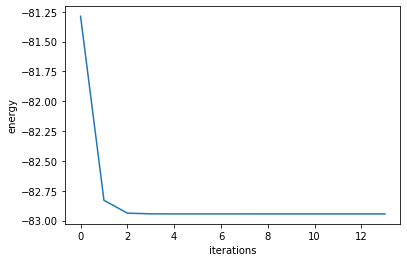
\includegraphics[width=1\textwidth]{convergence.png}
    \end{figure}
\end{frame}
\end{document}
